\documentclass[10pt]{article}
\usepackage[a4paper,margin=2cm]{geometry}
\usepackage{graphicx}\graphicspath{{fig/}}
\usepackage{amsmath,amssymb}
\usepackage[dvipsnames,table]{xcolor}
\usepackage{booktabs,caption,enumitem}
\usepackage{fontspec}
\setmainfont{Noto Serif CJK JP}
\XeTeXlinebreaklocale "ja"
\XeTeXlinebreakskip = 0pt plus 0.1pt minus 0.01pt
\usepackage[colorlinks=true,urlcolor=accent,linkcolor=accent]{hyperref}
\usepackage{titlesec}
\definecolor{ink}{HTML}{201A40}\definecolor{accent}{HTML}{2563EB}
\definecolor{grn}{HTML}{0E6B4F}\definecolor{mut}{HTML}{55556A}
\definecolor{discbg}{HTML}{FFF4D6}\definecolor{discfg}{HTML}{7A5A00}
\titleformat{\section}{\color{accent}\bfseries\large}{}{0pt}{}
\titlespacing{\section}{0pt}{11pt}{4pt}
\titleformat{\subsection}{\color{ink}\bfseries\normalsize}{}{0pt}{}
\titlespacing{\subsection}{0pt}{6pt}{2pt}
\setlist[itemize]{leftmargin=1.2em,itemsep=2pt,topsep=2pt}
\setlist[enumerate]{leftmargin=1.6em,itemsep=2pt,topsep=2pt}
\captionsetup{font={small,it},labelfont={color=mut},textfont={color=mut},skip=3pt}
\setlength{\parindent}{0pt}\setlength{\parskip}{4pt}\color{ink}\pagestyle{plain}
\newcommand{\keyword}[1]{\textbf{\color{accent}#1}}

\begin{document}
\noindent\colorbox{discbg}{\parbox{\dimexpr\linewidth-2\fboxsep\relax}{\color{discfg}\small\textbf{【ご注意】本ハンドアウトは機械翻訳によるものです。正確な内容については英語版を正としてご参照ください。}}}
\vspace{6pt}

{\LARGE\bfseries HyMeKo：構造化システムの表現と学習のための単一ハイパーグラフ基盤\par}
\vspace{2pt}{\color{accent}\itshape 宣言的なハイパーグラフ構造から、構造事前情報に基づく学習へ。\par}
\vspace{1pt}{\color{mut}\small 博士セミナー~~$\cdot$~~加藤研究室~~$\cdot$~~Csaba Hajdu~~$\cdot$~~2026年6月~~$\cdot$~~\emph{基礎的なグラフ理論から始める入門的ハンドアウト}\par}
\vspace{4pt}\hrule\vspace{6pt}

\section*{\color{accent}1.\quad はじめに --- なぜグラフか、そしてなぜそれだけでは不十分か}
世界の多くは\keyword{ものとものの関係}として自然に記述できる：信頼・不信を持つ人々、ロボットでつながった関節、分子で結合した原子、ニューラルネットワークで配線された層など。関係を表す標準的な道具が\emph{グラフ}である：点（\emph{頂点}）を線（\emph{辺}）でつないだもの。グラフは単純でよく理解されているため、至るところで使われる。

しかし通常の辺は\emph{ちょうど 2 つ}の頂点を結ぶのに対し、現実の関係の多くは\keyword{$n$ 項}である --- 複数のものを同時に束ねる。「Alice、Bob、Carol が共著した」は 1 つの三者関係であって、3 つの別々のペア関係ではない。これをグラフに押し込むと 3 本の辺を描き（図~\ref{fig:pvg} 左）、それが\emph{1 つの}共同事象だったという情報を静かに失う。\keyword{ハイパーグラフ}は、3 者すべてを含む単一の\emph{ハイパーエッジ}としてこれを保つ（図~\ref{fig:pvg} 右）。

本発表は一つの考えをその帰結まで追う。ハイパーグラフを基本対象として扱い、二つの問いを立てる：(i) 1 つの記述で多くのツール（シミュレータ、ロボット形式、モデリング言語、テンソルライブラリ）を駆動できるよう、構造化システムを\emph{どう記述}するか？ (ii) その同じ構造から\emph{どう学習}するか？ HyMeKo は単一の基盤で両方に答える --- \emph{フレームワークがコンパイルする構造が、モデルが推論する構造である}。

\begin{figure}[h]\centering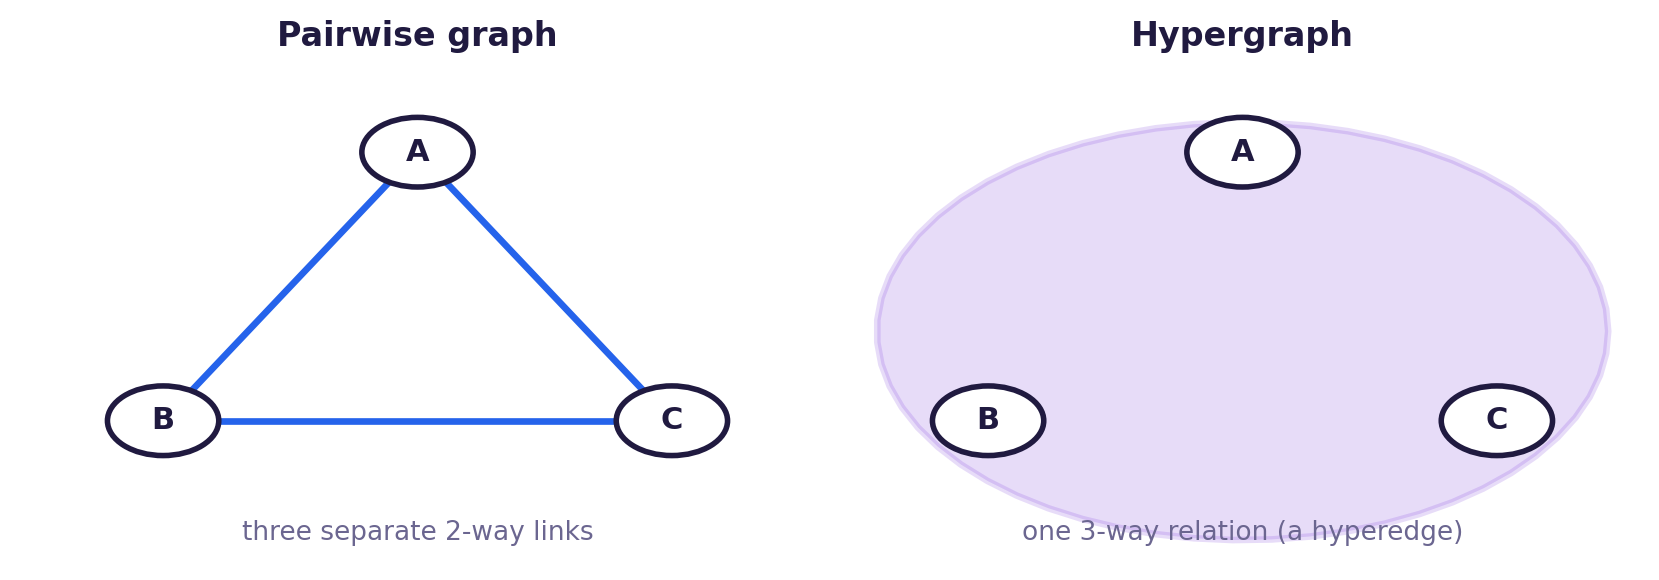
\includegraphics[width=.74\linewidth]{pairwise_vs_group.png}
\caption{ペアワイズグラフは 3 つの 2 者間リンクを、ハイパーグラフは 1 つの 3 者間関係を記録する。ペアワイズ符号化は群関係の同一性を失う。}\label{fig:pvg}\end{figure}

\section*{\color{accent}2.\quad グラフ理論の基礎の概観}
\subsection*{頂点・辺・近傍・次数}
\keyword{グラフ}は対 $G=(V,E)$ である：\keyword{頂点}（ノード）の集合 $V$ と\keyword{辺}の集合 $E$ で、各辺 $\{u,v\}$ は 2 つの頂点を結ぶ。辺に向きがあれば $(u\!\to\! v)$ と書き\emph{有向}グラフと呼ぶ。頂点 $v$ の\keyword{近傍} $N(v)$ は $v$ に結ばれた頂点であり、\keyword{次数} $\deg(v)=|N(v)|$ はその結合数である。図~\ref{fig:basic} では $\deg(B)=3$（近傍 $A,C,D$）。

\subsection*{ウォーク・パス・サイクル}
\keyword{ウォーク}は辺を端から端へつないだ列、例：$A\!-\!B\!-\!C$。その\emph{長さ}は辺数。\keyword{パス}は頂点を繰り返さないウォーク。\keyword{サイクル}は出発点に戻る閉じたパス、例：$A\!-\!B\!-\!D\!-\!E\!-\!A$。この 3 つ（ウォーク・パス・サイクル）は後で中心的役割を持つ：HyMeKo のモデルは構造をグラフの\emph{サイクル}から読む。

\subsection*{グラフを格納する二つの行列}
$n=|V|$ 頂点、$m=|E|$ 辺のとき、グラフは\keyword{隣接行列} $A\in\{0,1\}^{n\times n}$（$i,j$ が結ばれていれば $A_{ij}=1$）か、\keyword{接続行列} $B\in\{0,1\}^{n\times m}$（頂点 $i$ が辺 $e$ に属せば $B_{ie}=1$）として格納する。辺は\keyword{重み}（数）や、次に使う\keyword{符号}を持つこともある。

\begin{figure}[h]\centering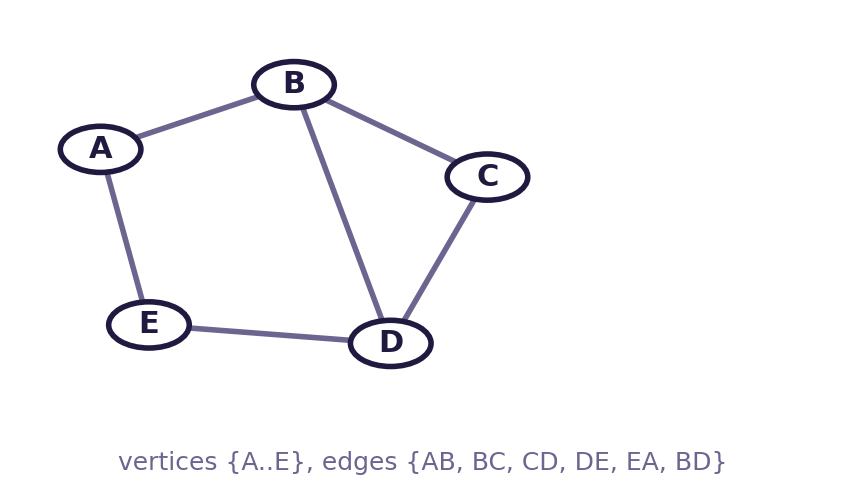
\includegraphics[width=.50\linewidth]{basic_graph.png}
\caption{小さな無向グラフ。例：パス $A\!-\!B\!-\!C$、サイクル $A\!-\!B\!-\!D\!-\!E\!-\!A$、$\deg(B)=3$。}\label{fig:basic}\end{figure}

\subsection*{もう少し別種のグラフ}
いくつかの特別な形が繰り返し現れる。すべての頂点対が結ばれたグラフは\keyword{完全グラフ}（$K_n$）で、辺数は $\binom{n}{2}$ と最も密。頂点が二つの側に分かれ辺が側を\emph{またぐ}ものだけ（側の内部には無い）なら\keyword{二部グラフ}で、ハイパー辺の符号付き「スター」形（$\S6$）はまさに二部グラフである。\keyword{木}はサイクルを持たない連結グラフで、$n$ 頂点なら辺はちょうど $n-1$ 本（連結で最も疎）。\keyword{部分グラフ}は頂点と辺の部分集合を残したもの。辺は\keyword{有向}（弧 $u\!\to\!v$、データフローや運動学連鎖）や\keyword{重み}付きにもでき、次に使う\keyword{符号}は $\pm1$ という最も単純な重みである。

\subsection*{連結性・距離・ラプラシアン}
ある二頂点はそれらを結ぶウォークがあれば\keyword{連結}、極大の連結部分が\keyword{連結成分}。二頂点間の\keyword{距離}は最短パスの長さ、その最大が\keyword{直径}。次数を対角に並べた\keyword{次数行列} $D$ から $L=D-A$ が\keyword{グラフラプラシアン}で、二階微分の離散版にあたり、その固有値はグラフがどれだけ連結で「滑らか」かを符号化する。ラプラシアン（と高次の Hodge 類縁）は後で再登場する：視覚版がハイパーグラフ上の曲率と流れを測る道具である。

\section*{\color{accent}3.\quad 符号付きグラフと構造的バランス}
\keyword{符号付きグラフ}は各辺に符号 $\sigma:E\to\{+,-\}$ を付ける --- 信頼／不信、友／敵、賛成／反対。構造的バランスは標準的な初級グラフ理論の範囲\emph{外}なので、丁寧に述べる。

\textbf{三角形の場合分け。} 3 人とその間の関係を考える。ラベルの付け替えを除くと符号パターンは 4 通り（図~\ref{fig:triads}）：全正 ($+\!+\!+$)、二正一負 ($+\!+\!-$)、一正二負 ($+\!-\!-$)、全負 ($-\!-\!-$)。三角形は 3 辺の符号の\emph{積}が $+$ のとき\keyword{バランスしている}。これは社会的直観（Heider, 1946）と一致する：「友の友は友」($+\!+\!+$) と「敵の敵は友」($+\!-\!-$) は心地よくバランスし、「友の友が敵」($+\!+\!-$) や「三者相互に敵」($-\!-\!-$) は緊張しアンバランス。

\textbf{三角形から任意のサイクルへ。} 同じ規則が任意のサイクルに拡張する：$\sigma(C)=\prod_{e\in C}\sigma(e)$、これが $+$ のときバランス。

\textbf{Harary のバランス定理（1953）。} 符号付きグラフが\emph{完全に}バランスするのは、頂点を二つの陣営に分け、すべての $+$ 辺が陣営\emph{内}に、すべての $-$ 辺が陣営\emph{間}に来るようにできるとき、ちょうどそのとき --- 「二派閥：内は友、間は敵」。

\textbf{弱バランスと、実グラフはどれだけバランスしているか。} Heider の原概念（1946）は心理学的、Cartwright--Harary（1956）が上記のグラフ理論形を与えた。Davis（1967）はこれを緩めた：\emph{ちょうど 1 本}の負辺を持つサイクルが無いグラフは\keyword{弱バランス}（クラスタ化可能）で、全負三角形（三者が三陣営に分かれ相互に敵対）を許し、頂点は二つでなく $k\ge2$ 陣営に分割できる。実在の社会・信頼ネットワークが完全にバランスすることはない。そのずれの標準的尺度が\keyword{フラストレーション（線）指数} --- バランスに到達するのに必要な最小の辺符号反転数。経験的にこれらはバランスに近く、その近さこそが欠損符号の問いを解けるものにしている。

\textbf{なぜ予測を駆動するか。} 実ネットワークは\emph{近似的}にしかバランスしないが、バランスへの引力は強いため、\emph{欠損}辺の符号は通常、それを通るサイクルをバランスに保つ符号である。\keyword{符号付きリンク符号予測}は一部の辺符号を隠して復元させる。HSiKAN と G\"omb はこのサイクルバランス信号のソフトでデータ駆動な版を学習する --- そして構造を通じて答えを覗かず\emph{誠実に}行うことが本発表の通底テーマである。

\begin{figure}[h]\centering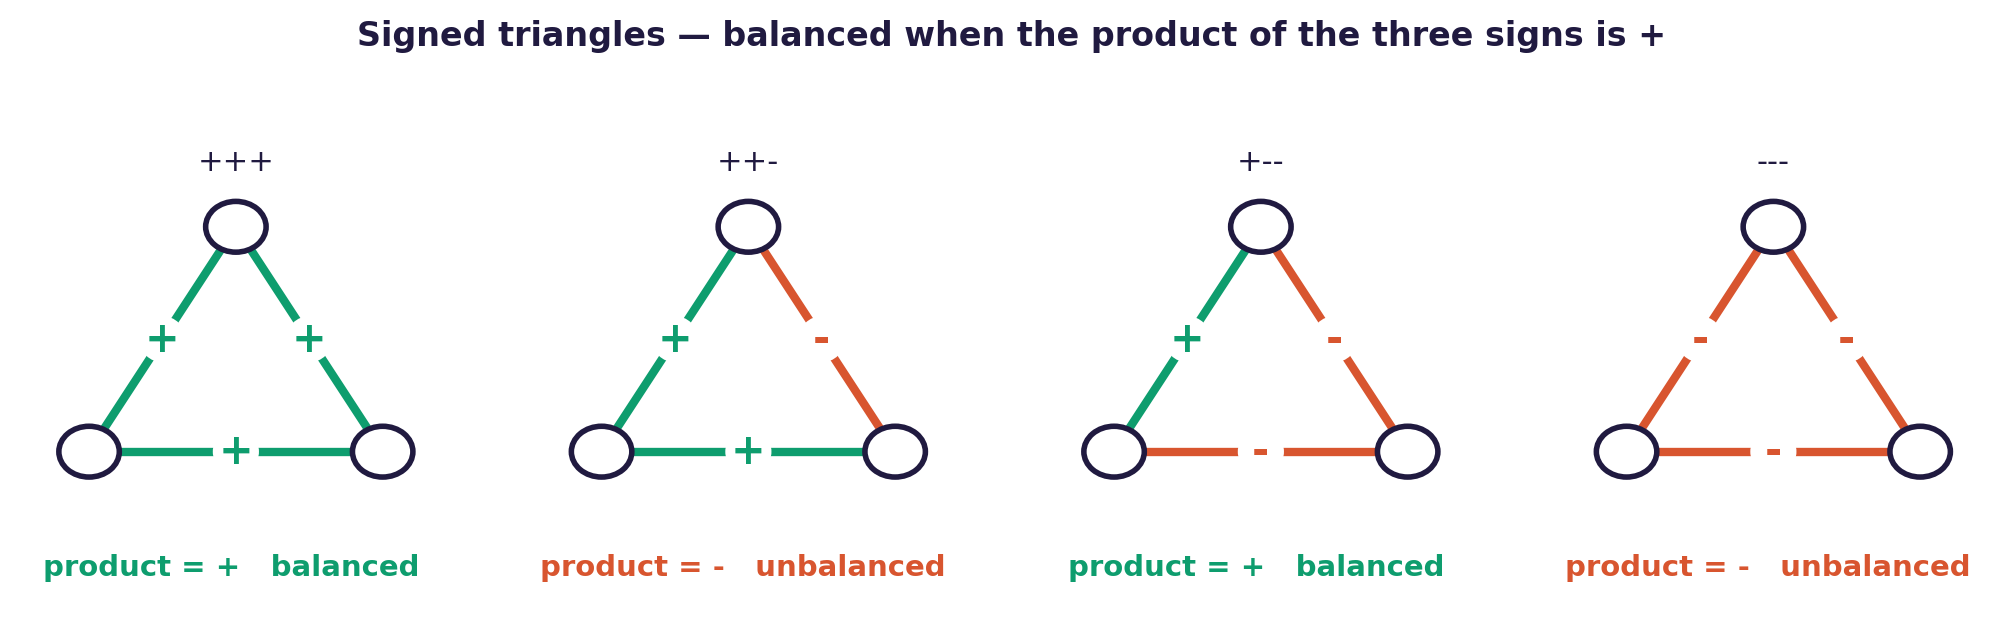
\includegraphics[width=.92\linewidth]{balance_triads.png}
\caption{4 つの符号付き三角形。バランス $\Leftrightarrow$ 3 辺の符号の積が $+$（$+\!+\!+$ と $+\!-\!-$ の場合）。他の 2 つはアンバランス。}\label{fig:triads}\end{figure}

\begin{figure}[h]\centering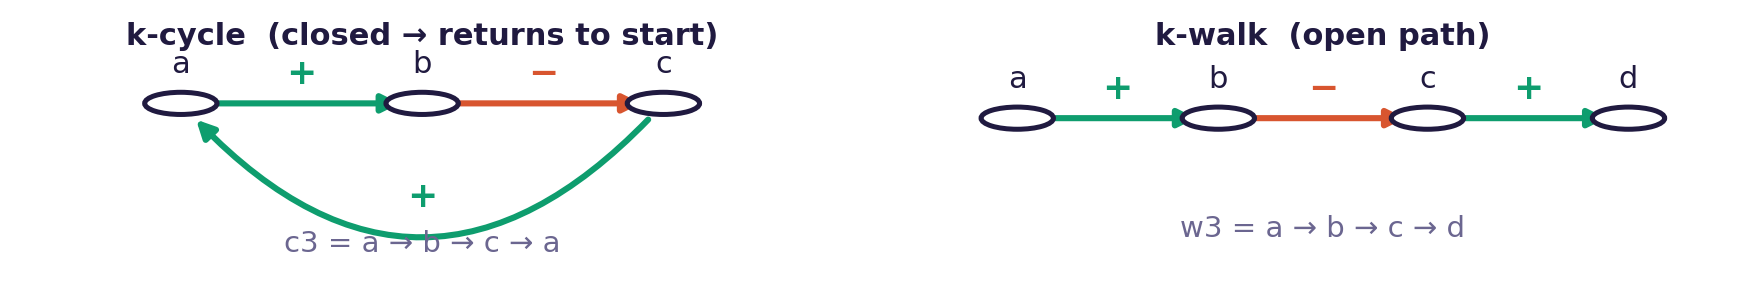
\includegraphics[width=.80\linewidth]{kcw.png}
\caption{$k$-サイクル（閉：始点に戻る）と $k$-ウォーク（開いた経路）。緑 $+$、赤 $-$。サイクルの符号は辺の符号の積。}\end{figure}

\section*{\color{accent}4.\quad グラフからハイパーグラフへ}
\keyword{ハイパーグラフ} $H=(V,E)$ は「端点は 2 つ」という規則を緩める：各\keyword{ハイパーエッジ} $e\in E$ は任意サイズ $|e|=k$（\emph{アリティ}）の頂点部分集合 $e\subseteq V$ である。$k=2$ で通常のグラフに戻る。$\bar d$ は平均アリティ。ハイパーグラフを行列ライブラリで扱える形に戻す標準的な方法が二つある：
\begin{itemize}
\item \keyword{スター（Levi/Berge）展開。} ハイパーエッジごとに「ハブ」ノードを 1 つ加え、その構成頂点に結ぶ。符号付き頂点×ハイパーエッジ接続は $B\in\{-1,0,+1\}^{|V|\times|E|}$。コストは\keyword{$O(|E|\,\bar d)$} --- アリティに線形。
\item \keyword{クリーク展開。} 各ハイパーエッジをクリーク（全構成頂点を総当たりで結ぶ）に置き換える。通常のグラフに戻るがコストは\keyword{$O(|E|\,\bar d^{2})$} --- 二次の「膨張」（$k$ 項関係が $\binom{k}{2}$ 本の辺になる）。
\end{itemize}
HyMeKo はコストを線形に保ち各関係の同一性を保つため、スター展開を用いる（図~\ref{fig:levi}）。

\begin{figure}[h]\centering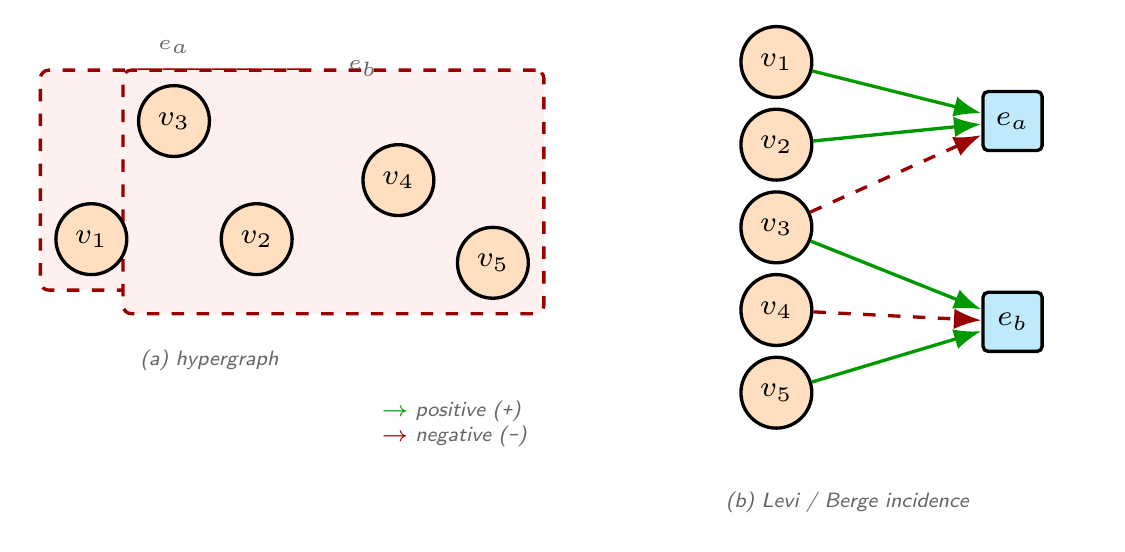
\includegraphics[width=.62\linewidth]{levi.png}
\caption{符号付きハイパーグラフ（$v_1\dots v_5$ 上のハイパーエッジ $e_a,e_b$）と、その Levi/Berge 接続（スター展開）。緑 $+$、赤 $-$。}\label{fig:levi}\end{figure}

\section*{\color{accent}5.\quad Kolmogorov--Arnold 表現と KAN}
古典的定理（Kolmogorov--Arnold, 1957）によれば、多変数の任意の連続関数は\emph{一変数}関数と加算だけで書ける：
\[ f(x_1,\dots,x_n)=\sum_{q=0}^{2n}\Phi_q\!\Big(\sum_{p=1}^{n}\psi_{q,p}(x_p)\Big). \]
\keyword{Kolmogorov--Arnold ネットワーク（KAN）}はこれを学習可能なモデルにする：（ReLU のような）固定活性化を\emph{ノード}に置く代わりに、\emph{学習可能な一変数関数を辺}に置く。各関数は\keyword{スプライン}（少数の制御点に固定された滑らかな曲線、ここでは Catmull--Rom スプライン、図~\ref{fig:cr}）で表す。HSiKAN はこの学習可能スプラインをハイパーグラフの\emph{符号付きサイクル／ウォークのタプル}に置き、グラフ自身の構造をモデルの帰納的事前情報にする。

なぜこの定理は驚きか。本当に多変数な操作は\emph{加算}だけでよい、というのだ：すべての「形」は一変数関数 $\psi_{q,p}$ と $\Phi_q$ に宿る。KAN はこれを文字通り実装する。従来の \keyword{MLP} は活性化（ReLU, tanh）を固定し辺の\emph{線形重みを学習}するが、KAN は逆 --- 辺が\emph{学習可能な関数}を担い、別個の重み行列は無い。関数のパラメータは少数の\keyword{制御点}の高さにすぎず、\keyword{Catmull--Rom} スプラインがそれらの点を\emph{通って}局所制御で滑らかに補間する（一点を動かしても近傍しか変わらない）ので、曲線は解釈可能で評価も安価なまま。

これは我々の設定によく合う。符号付きサイクルの寄与は特徴タプルの概ね滑らかな関数であり、どのサイクル長が効くかを事前に仮定せず\emph{学習}させたい。符号付きサイクル／ウォークのタプルごとに学習可能スプラインを一つ置くことで、グラフ自身の構造が帰納的事前情報になる --- モデルの容量は汎用の密ネットワークでなく、構造から符号への写像の形に費やされる。

\begin{figure}[h]\centering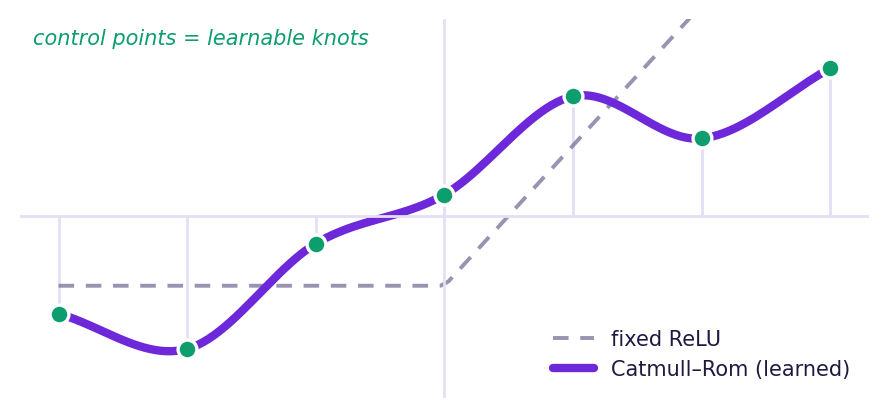
\includegraphics[width=.40\linewidth]{cr.png}
\caption{学習可能な Catmull--Rom スプライン活性化（固定 ReLU との対比）— KAN の基本要素。}\label{fig:cr}\end{figure}

\section*{\color{accent}6.\quad 単一基盤、二つの成果}
宣言的な \texttt{.hymeko} ソースは、SIMD レキサと LALRPOP パーサを経て、Blake3 内容ハッシュによる同一性を持つ単一の正準ハイパーグラフ IR へコンパイルされる。この単一 IR から、多数のターゲット形式の出力と、構造事前情報に基づく学習スタックへの供給の双方が行われる。

\begin{figure}[h]\centering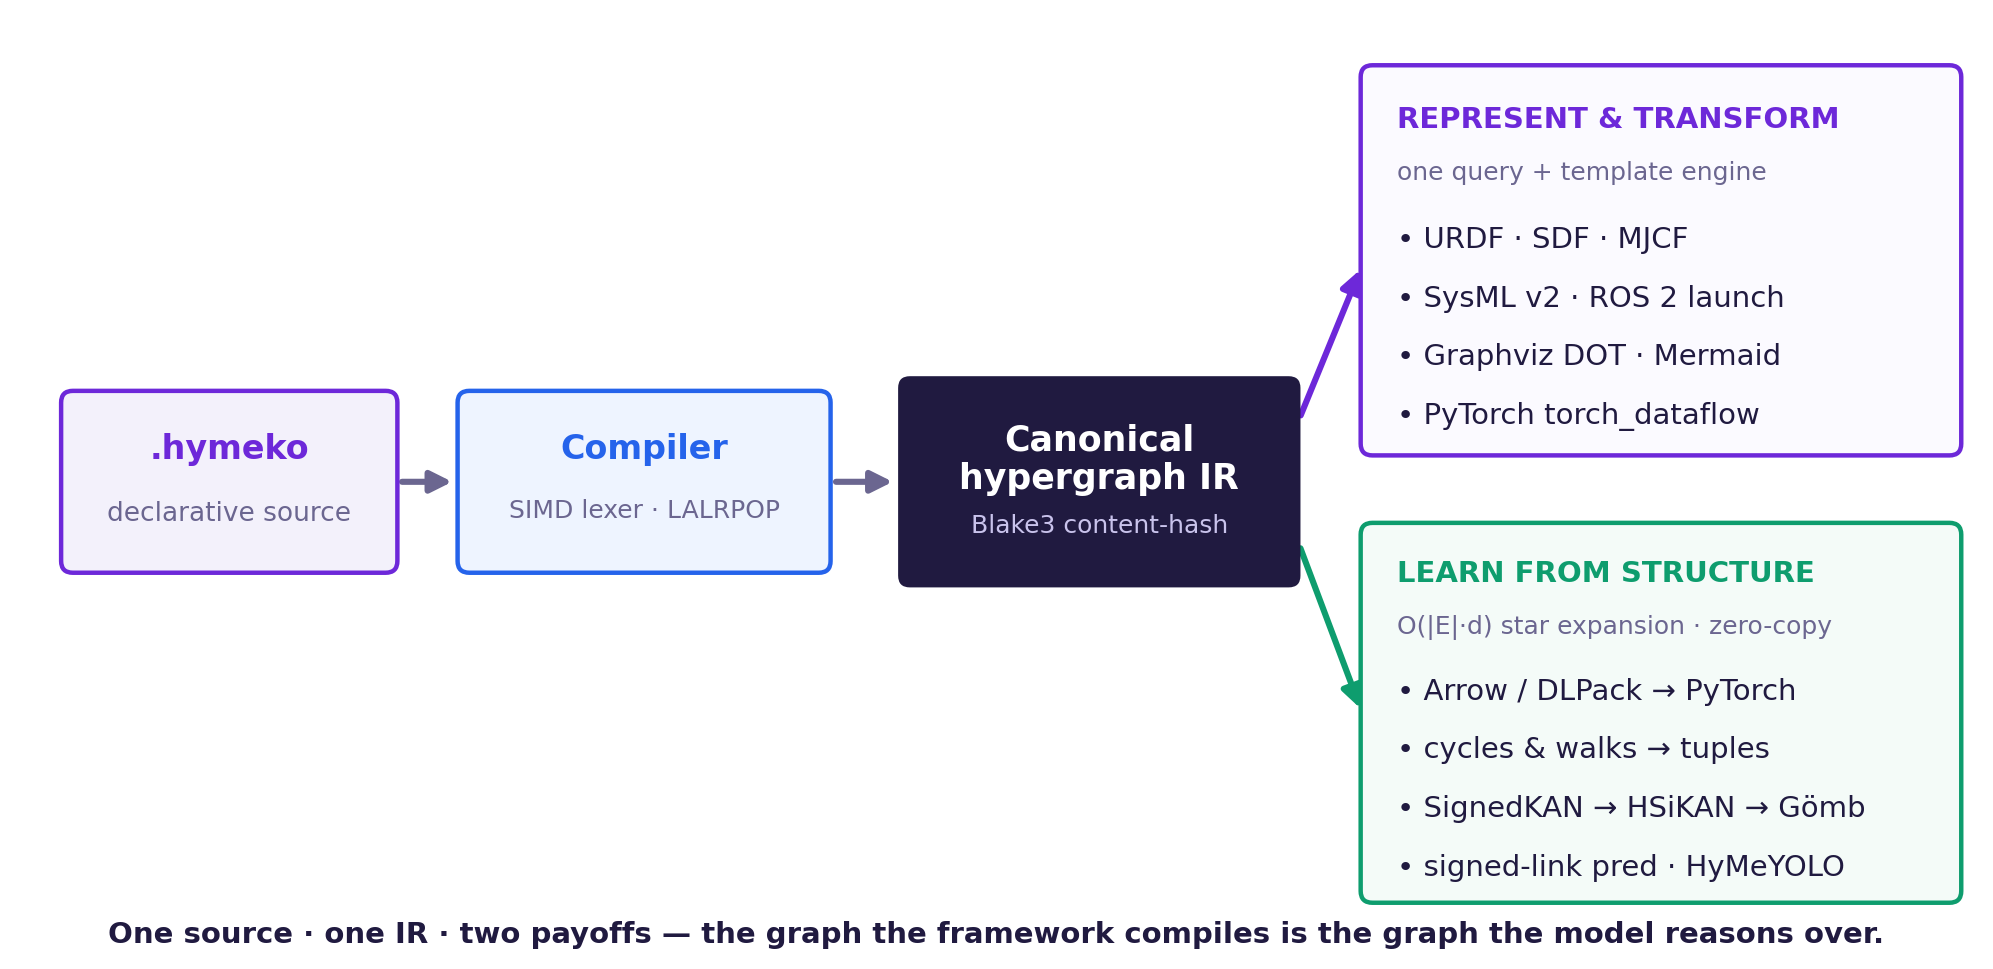
\includegraphics[width=.95\linewidth]{workflow.png}
\caption{HyMeKo のワークフロー：単一ソース $\to$ 単一の正準 IR $\to$ 二つの成果（表現・変換／構造からの学習）。}\end{figure}

\subsection*{仕組み --- パイプライン}
\begin{enumerate}
\item \textbf{記述} --- 宣言的な \texttt{.hymeko} ソース。ジオメトリ・色・語彙は重複させず参照で再利用。
\item \textbf{コンパイル} --- SIMD レキサ ＋ LALRPOP パーサが Blake3 内容ハッシュ同一性を持つ単一の正準ハイパーグラフ IR を生成。
\item \textbf{表現} --- 単一のクエリ＋テンプレートエンジンが URDF・SDF・MJCF・SysML\,v2・ROS\,2 launch・DOT・Mermaid・PyTorch をビュー間整合で出力。
\item \textbf{ストリーム} --- $O(|E|\,\bar d)$ のスター展開を PyTorch へゼロコピー（Iceoryx2 / Arrow / DLPack）。トポロジハッシュのゲート（$<100\,\mu$s）が構造と重みを分離。
\item \textbf{列挙} --- 訓練エッジ上の符号付き $k$-サイクルと $k$-ウォークが構造タプル（$c_3\cdot c_4\cdot c_5\cdot w_2\cdot w_3$）になる。
\item \textbf{学習} --- SignedKAN $\to$ HSiKAN $\to$ Gömb（Clifford-FIR $\to$ HSiKAN-CR $\to$ CPML）。Catmull--Rom スプライン、エッジごとの CR ハイウェイ（\texttt{edge\_cr}）、四元数符号アテンション。
\item \textbf{監査} --- リーク検査済みの厳格なプロトコル：サイクルプールはテストエッジ符号を見ない。ラベルシャッフルで偶然（$0.540$）まで低下、5シード対応差。
\end{enumerate}

\section*{\color{accent}7.\quad 第 I 部 --- フレームワーク}
\begin{itemize}
\item 参照による再利用を備えた宣言的 DSL：ジオメトリ（と色）を一度だけ定義し visual と collision の両方から参照。運動学の語彙は一度だけインポート。
\item Blake3 内容ハッシュ同一性を持つ正準ハイパーグラフ IR — 同型な記述は単一のフィンガープリントを共有。
\item 単一のクエリ＋テンプレートエンジンが URDF / SDF / MJCF / SysML\,v2 / ROS\,2 / DOT / Mermaid / PyTorch を出力 — 再コンパイル不要。
\item Iceoryx2 / Arrow / DLPack による PyTorch へのゼロコピー連携。トポロジハッシュゲート（$<100\,\mu$s）。
\end{itemize}

\begin{table}[h]\centering\small
\caption{同一の 50ノード / 50エッジ / 密度0.30 のハイパーグラフでのスター対クリーク材料化 --- \S4 の線形 対 二次コストを数値で。}
\begin{tabular}{lrr}\toprule
材料化 & 非ゼロ要素 & 抽出時間\\\midrule
スター \;$O(|E|\,\bar d)$ & 1{,}498 & 79.7 ms\\
クリーク \;$O(|E|\,\bar d^{2})$ & 10{,}991 & 496 ms\\\bottomrule
\end{tabular}\end{table}

\begin{table}[h]\centering\small
\caption{同一ロボットのソース文字数。HyMeKo はジオメトリ／色を参照で再利用、URDF は visual と collision を重複記述。$^\dagger$\emph{完全な} HyMeKo ソースは関節制御インタフェース・センサ・Gazebo/ros2\_control デプロイも\emph{単一}ファイルに含む --- 素の URDF/MJCF では不可能であり、運動学のみの MJCF 値は等価比較ではない。}
\begin{tabular}{lrrr}\toprule
運動学構造 & HyMeKo & URDF & MJCF\\\midrule
2関節接続 & 71 & 164 & 91\\
SCARA & 101 & 252 & 129\\
6自由度アーム（運動学のみ） & 2{,}779 & 5{,}088 & 1{,}733\\
\addlinespace
6自由度アーム（全体：制御・センサ含む）$^\dagger$ & \textbf{6{,}134} & 複数ファイル & 機構のみ\\\bottomrule
\end{tabular}\end{table}

\section*{\color{accent}8.\quad 第 II 部 --- 構造からの学習}
\begin{itemize}
\item 列挙された符号付き $k$-サイクルと $k$-ウォークが帰納的特徴（タプル）になる — 事前情報としての構造。
\item SignedKAN $\to$ HSiKAN $\to$ Gömb は固定活性化を学習可能な Kolmogorov--Arnold（Catmull--Rom）スプラインで置換。HSiKAN はアリティ混合器、エッジごとの Catmull--Rom ハイウェイ（\texttt{edge\_cr}）、四元数符号アテンションを追加。
\item Gömb は厳格な三シェルのカスケード — Clifford-FIR（四元数／多元数の符号付きフィルタ）$\to$ HSiKAN-CR $\to$ CPML — で、サイクルプールは訓練エッジのみで列挙。
\item 視覚向け変種は Forman--Ricci 曲率と Hodge 分解（$\partial^2{=}0$、1次ホモロジー、離散リッチフロー）を伴う Clifford-FIR / 四元数機構を追加。
\end{itemize}

\begin{figure}[h]\centering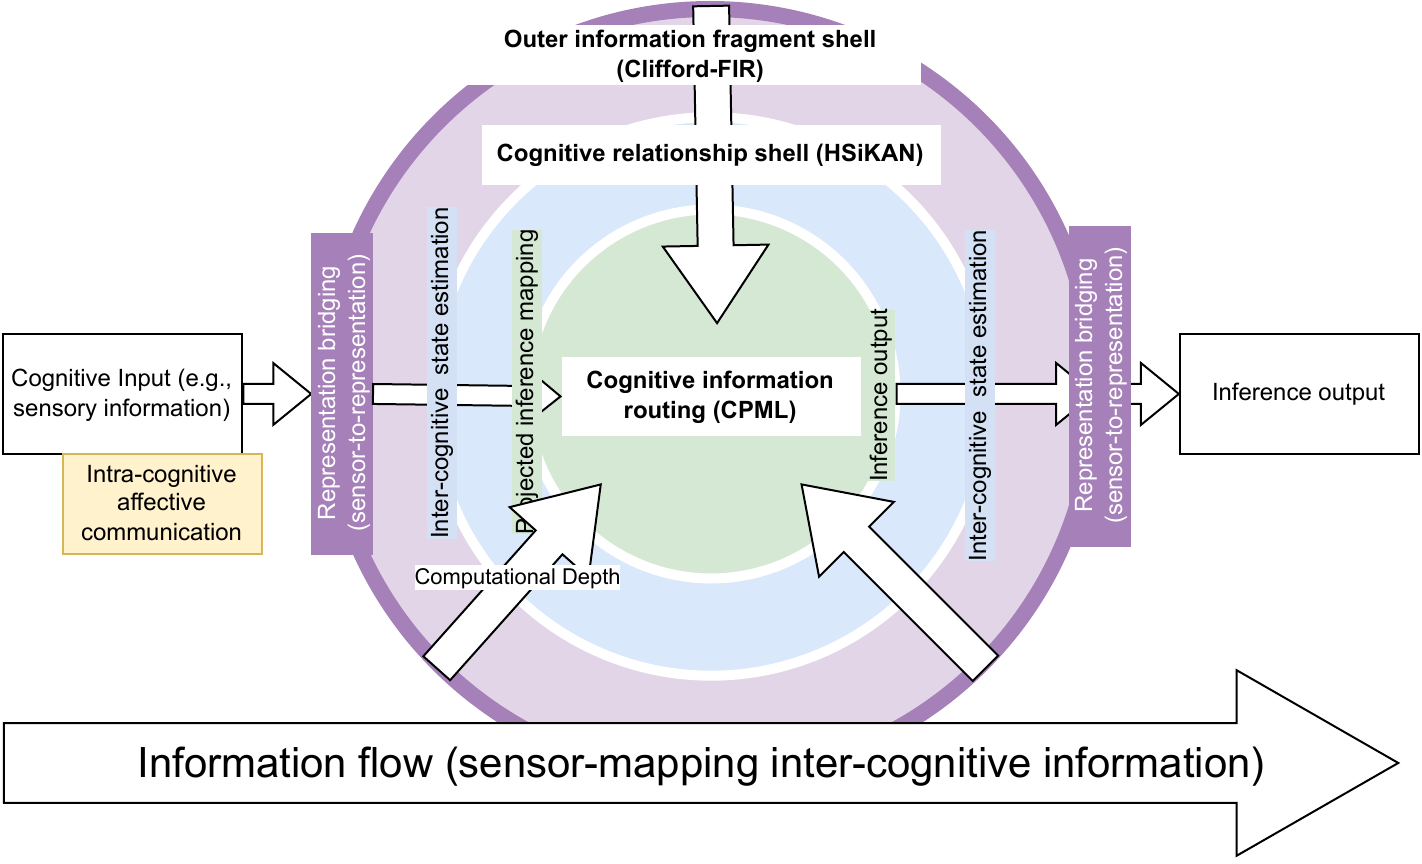
\includegraphics[width=.55\linewidth]{gomb.png}
\caption{Gömb の構造事前情報カスケード（Clifford-FIR $\to$ HSiKAN-CR $\to$ CPML）。}\end{figure}

\section*{\color{accent}9.\quad 主な結果（誠実な提示）}
\begin{itemize}
\item 低コスト（パラメータ約 $\tfrac14$）で競争力があり一部最先端、Epinions では真に優位 — 一律の SOTA 主張ではない。（transductive 慣行では調整済み構成が Bitcoin で $0.996/0.993$。）
\item 効率：約 30k パラメータ。強みはパラメータあたり精度。系列内の順伝播差（h4 対 h16、同一デバイス）は CPU 約 3.5$\times$、CUDA 約 1$\times$。
\item 転移：HyMeYOLO は mAP$_{50}\approx0.90$（ReLU バックボーンと同等）。運動学はトポロジのみから約 5\,cm で復元。
\item 方法論：ラベルシャッフル診断（Gömb $\to 0.540$ = 偶然）、5シード対応差、全数値がディスク上の成果物に対応。
\end{itemize}

\begin{table}[h]\centering\small
\caption{符号付きグラフのリンク予測、ホールドアウト test ROC-AUC（5シード、Gömb-strict）。ベースラインは公表値。}
\begin{tabular}{lccc}\toprule
データセット & \textbf{Gömb-strict（本研究）} & SGCN & SiGAT\\\midrule
Bitcoin-$\alpha$ & \textbf{0.897} & 0.929 & 0.903\\
Bitcoin-OTC & \textbf{0.915} & 0.942 & 0.932\\
Slashdot & \textbf{0.902} & 0.919 & ---\\
Epinions & \textbf{0.943}（FT 0.953） & --- & $\approx$0.95\\\bottomrule
\end{tabular}\end{table}

\section*{\color{accent}10.\quad 新しい結果 --- Cayley ローター埋め込み（2026-06-16）}
パラメータ一定・帰納的・リークのない埋め込み：各項目の埋め込みは、球面上の一つの共有基準ベクトルを（Cayley 写像による Clifford ローターで）学習回転したものであり、ノードごとの参照表を持たない。パラメータが増大するベースライン（DADSGNN）に対し約 9--16$\times$ 少ないパラメータで同等の性能を示し、ラベルシャッフルでは偶然（約 0.50）まで低下する。

\begin{figure}[h]\centering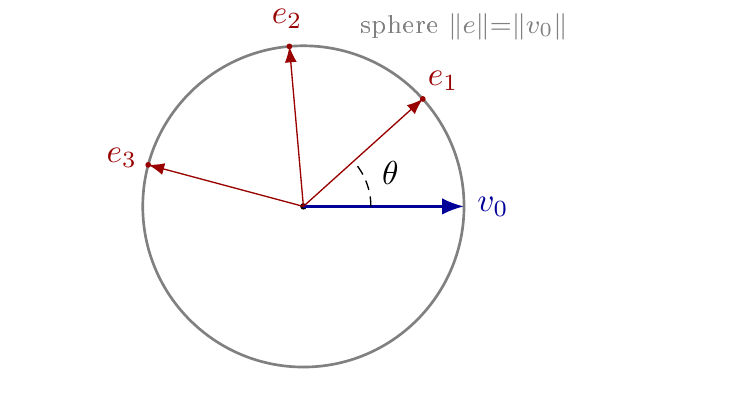
\includegraphics[width=.34\linewidth]{rotor.png}
\caption{ローター埋め込み：各項目は球面上の一つの基準ベクトルの回転で、角度が類似度。}\end{figure}

\begin{table}[h]\centering\small
\caption{符号付きリンク予測の test ROC-AUC、5シード。ローターはパラメータ一定、ベースラインは増大。出典：\texttt{reports/rotor\_multiseed\_20260616.jsonl}。}
\begin{tabular}{lcccc}\toprule
データセット & \textbf{Rotor AUROC} & \textbf{Rotor params} & DADSGNN AUROC & DADSGNN params\\\midrule
Bitcoin-$\alpha$ & \textbf{0.867 $\pm$ 0.011} & \textbf{15.8k} & 0.860 $\pm$ 0.011 & 142k\\
Bitcoin-OTC & \textbf{0.894 $\pm$ 0.006} & \textbf{15.8k} & 0.880 $\pm$ 0.007 & 209k\\
wiki\_elec & \textbf{0.885 $\pm$ 0.002} & \textbf{15.8k} & 0.896 $\pm$ 0.007 & 249k\\\bottomrule
\end{tabular}\end{table}

\section*{\color{accent}11.\quad 貢献と連絡先}
\begin{itemize}
\item 正準ハイパーグラフ基盤 — DSL と内容ハッシュ付き IR。単一ソースから多数のターゲットへ。
\item 構造事前情報に基づく学習系列 — 帰納的特徴としてのサイクルとウォーク（SignedKAN / HSiKAN / Gömb）、厳格なリーク検査つき。同一の IR が工学的変換と学習基盤の双方を担う。
\end{itemize}
Csaba Hajdu~~$\cdot$~~加藤研究室。\quad コードとドキュメント：\url{https://github.com/kyberszittya/hymeko_framework_rust}

\clearpage
\section*{\color{accent}12.\quad スライドごとの詳細解説}
本節は発表をスライド単位で写し、セミナー後も単独で読めるようにする。各項目はスライドが何を示しなぜそこにあるかを述べる。概念的なスライド（ハイパーグラフ、バランス、$k$-列挙、漏洩）には少し紙幅を割き、節の区切りは一行にとどめる。

\subsection*{Slide 1 --- Title}
冒頭スライドは発表タイトル、会場（加藤研究室）、発表者、日付を示し、発表全体を貫く主題「単一基盤、二つの成果」を提示する。同じハイパーグラフという対象が、システムを\emph{記述}することと、そこから\emph{学習}することの両方に使えるという考えである。

\subsection*{Slide 2 --- Contributions}
詳細に入る前に、二つの結合した貢献を提示する。(i) 正準ハイパーグラフ\emph{基盤}（DSL と内容ハッシュ付き IR）。(ii) グラフのサイクルを読む構造事前情報の\emph{学習}系列。要点は両者が\emph{同一}の IR に立脚すること。発表の四区分（問題 $\to$ 枠組み $\to$ 学習 $\to$ 証拠）も示す。

\subsection*{Slide 3 --- HyMeKo, in brief}
初学者向けの一段落の見取り図：HyMeKo はハイパーグラフ記述を正準中間表現にコンパイルし、その単一表現から多数の形式へ\emph{変換}し、かつそこから\emph{学習}する Rust フレームワークと小さな宣言的言語である。

\subsection*{Slide 4 --- Why hypergraphs?}
動機。現実の関係はしばしば 3 つ以上を同時に束ねる（$n$ 項）。これを通常の（ペアワイズ）グラフに押し込むと各関係の同一性が失われ表現が膨張する。$K_5$ の図がコストを具体化する：1 つの $k$ 項関係をペアワイズ辺にすると $\binom{k}{2}$ 本必要 --- $O(d^2)$ のクリーク膨張。聴衆に持ち帰ってほしい要点は単純：$k$ 項関係は一つの対象であり、ペアワイズ符号化は辺数を増やすうえに、それらの辺が元来一体だったことを忘れる。

\subsection*{Slide 5 --- Typical hypergraphs}
正準例のギャラリー --- Fano 平面、一般のハイパーグラフ、完全 3 一様 $K_4^{(3)}$、ひまわり --- それぞれハイパーエッジにラベルを付け、\texttt{.hymeko} ソースを併記。「ハイパーグラフ」を具体化し、これらが実在するコンパイル可能なフィクスチャであることを示す。

\subsection*{Slide 6 --- A hyperedge and its signed incidence}
単一のハイパーエッジに注目し、その符号付き Levi/Berge 接続 --- ハブを 1 つ持つ二部「スター」形 --- を緑 $+$、赤 $-$ で示す。以降すべてが立脚する表現である。

\subsection*{Slide 7 --- One substrate, two payoffs}
主張スライド。単一の正準 IR が\emph{表現}（多形式出力）と\emph{学習}（構造事前情報）の双方を担う。よってフレームワークがコンパイルするグラフが、文字どおりモデルが推論するグラフであり、乖離しうる別個の成果物にならない。

\subsection*{Slide 8 --- What HyMeKo describes}
基盤が実際に扱う領域を概観：ロボット機構と運動学、モデルベースシステムズエンジニアリング／SysML、符号付きソーシャルグラフ、ニューラルネットのデータフロー --- 抽象化が一分野専用でなく一般的であることの証左。

\subsection*{Slide 9 --- Goals at two levels}
目標を\emph{言語}レベル（人間に優しく再利用可能な DSL）と\emph{基盤}レベル（高速コンパイラ、正準 IR、ゼロコピーランタイム）に分け、各々で貢献を評価できるようにする。

\subsection*{Slide 10 --- The HyMeKo workflow}
システム全体の一枚地図：\texttt{.hymeko} ソースがレキサ／パーサを経て正準 IR となり、二つの成果 --- 一方は表現・変換、他方は構造からの学習 --- へ展開する。以降すべての心的モデル。

\subsection*{Slide 11 --- Part I divider}
フレームワーク編を開く区切り。

\subsection*{Slide 12 --- A declarative language for hypergraphs}
DSL の導入：ハイパーエッジは第一級、ノードは階層パスに入れ子化、アークは $+/-$ 符号と役割タグを持つ。\emph{コンパイル可能}な \texttt{robot.hymeko} 例が要点を示す --- ジオメトリ（と色）を一度定義し、visual と collision の両方から\emph{参照}し、重複させない。

\subsection*{Slide 13 --- From source text to a hypergraph IR}
コンパイラの流れ：SIMD 加速レキサと LALRPOP（LR(1)）パーサが、ノードに Blake3 内容ハッシュ同一性を持つ正準 IR を生成（同型記述は単一フィンガープリントを共有）。シンボルインターン、スター／クリーク展開を随時利用。

\subsection*{Slide 14 --- Star vs clique}
$\S4$ の線形対二次を、固定した 50ノード / 50エッジ / 密度0.30 のハイパーグラフで定量化：スター展開は非ゼロ 1{,}498、79.7\,ms、クリーク展開は 10{,}991、496\,ms。二つのヒートマップが密度差を可視化。

\subsection*{Slide 15 --- A zero-copy bridge to the GPU}
スター展開を無コピーで PyTorch へ流す仕組み --- Iceoryx2 共有メモリ、Apache Arrow、DLPack --- と、トポロジハッシュゲート（$<100\,\mu$s）が構造更新と重みストリームを区別し、変化分のみを再送することを説明。

\subsection*{Slide 16 --- Query-driven transforms}
クエリ＋テンプレートエンジンが単一 IR から URDF、SDF、MJCF、SysML、PyTorch モジュールを出力。$N\times M$ のペア変換器問題がハブ＆スポークに収束し、出力される各ビューは互いに整合が保証される。

\subsection*{Slide 17 --- How compact is the DSL?}
6 自由度アームでの文字数比較（HyMeKo 対 URDF 対 MJCF）。誠実な枠組み：HyMeKo はジオメトリ／色を参照で再利用し URDF は visual と collision を重複。完全な\emph{デプロイ}系は単一 \texttt{.hymeko} 対 複数ファイルの ROS/Gazebo バンドル。MuJoCo で生成ロボットを描いたスクリーンショット付き。

\subsection*{Slide 18 --- Built like a system, not a script}
コードを支える工学的規律：SysML\,v2 モデル、読み取り専用コアを示す \texttt{CORE.YAML} 保護契約、計画優先のワークフロー --- システムとして保守されている証左。

\subsection*{Slide 19 --- Part II divider}
サイエンス編を開く区切り。

\subsection*{Slide 20 --- From structure to inductive prior}
第 I 部から第 II 部への蝶番：グラフのサイクルとウォークを構造特徴となるタプルに変え、サイクルアリティ\emph{コンパス}を機構族のフィンガープリントとして示す。モデル自体も \texttt{.hymeko} で記述される点に注意。

\subsection*{Slide 21 --- The model family}
モデルの発展を提示し、デプロイ構成 --- Clifford-FIR $\to$ HSiKAN-CR $\to$ CPML --- を名付け、以降の詳細スライドの地図とする。

\subsection*{Slide 22 --- G\"omb: a strict cascade}
三シェル（Clifford-FIR $\to$ HSiKAN-CR $\to$ CPML）と、誠実さを生む設計上の一点：サイクルプールは\emph{訓練}エッジのみで列挙されるため、テストエッジの符号が漏れ込めない --- ラベルシャッフルで偶然まで低下する。

\subsection*{Slide 23 --- What is k-enumeration?}
構造特徴そのものの説明：各アリティの符号付き $k$-サイクルと $k$-ウォークの列挙。閉じたサイクルと開いたウォークの図解付き。なぜこれがボトルネックか、どう有界化するか（頂点ごと top-$k$ スコアリング、アリティごとの上限）も説明。要するに $k$-列挙は生のトポロジーをスプライン層が消費できる固定幅特徴に変える手段であり、上限が密グラフでの扱いやすさを保つ。

\subsection*{Slide 24 --- Inside HSiKAN}
中間シェルを開く：Catmull--Rom スプライン活性化、アリティ混合器で融合される混合アリティ層、四元数符号アテンション、そして強い参照構成であるエッジごとの Catmull--Rom ハイウェイ（\texttt{edge\_cr}）。

\subsection*{Slide 25 --- HSiKAN, learned}
概略図でなく実推論の出力を示す：学習されたアリティ重みベクトル $\alpha_k$（どのサイクル長に依存するか）と、AUROC を伴う ROC 曲線。

\subsection*{Slide 26 --- Clifford-FIR and quaternion machinery}
外側シェル：\texttt{hymeko\_clifford} 自動微分バックエンド（多元数、ブレード積、$(p,q)$ 計量）上の並列 Clifford-FIR フィルタバンク。Forman 曲率、Hodge 分解、Bochner --- V1$\to$V4$\to$IT の類推で提示。

\subsection*{Slide 27 --- Signed-graph link prediction results}
主要結果：G\"omb-strict プロトコルでのデータセット横断ホールドアウト 5 シード ROC-AUC を、公表ベースラインと並べて表と図で提示。誠実な枠組み（低コストで競争力があり一部最先端、Epinions で真に優位、一律 SOTA 主張ではない）。

\subsection*{Slide 28 --- SOTA range --- at a fraction of the cost}
効率の物語：約 30k パラメータ、パラメータあたり精度で測る優位、系列内の幅差（h4 対 h16）、大規模多シード実行に用いた Komondor スーパーコンピュータへの言及。

\subsection*{Slide 29 --- New result: Cayley-rotor embeddings}
最新結果：パラメータ一定・帰納的・リークのない埋め込み。各項目は球面上の一つの共有基準ベクトルの学習回転（Cayley 写像による Clifford ローター）。増大型 DADSGNN に対し 9--16$\times$ 少ないパラメータで同等、ラベルシャッフルで偶然まで低下。

\subsection*{Slide 30 --- What is leakage?}
プロトコルが防ぐ失敗様式の教示スライド：transductive $\sigma$-リーク --- モデルがテストエッジの符号を構造を通じて密かに読み、予測でなくカンニングで好成績を出す現象。具体的には、サイクルプールを全辺で構築すると、ホールドアウト辺を通るサイクルがすでにその符号を「見て」しまい、高スコアは汎化でなく記憶を測る --- だから次のスライドはこれを排除する話になる。

\subsection*{Slide 31 --- Honesty as a protocol}
評価姿勢の表明：報告する全数値がディスク上の成果物に対応し、主張は保守的に枠付けする厳格プロトコル。

\subsection*{Slide 32 --- How we know it isn't leakage}
前スライドの証拠：訓練エッジの符号をシャッフルして再学習すると G\"omb は $0.540$（偶然）に落ちる。これは技能が記憶テーブルでなく真の構造に由来することを示す。論理は対照実験そのもの：構造を壊す（符号をシャッフルする）と、技能が構造由来なら消えるはず --- 実際に偶然線まで落ちるので、モデルが使う信号はバランスのパターンであって漏れたラベルではない。

\subsection*{Slide 33 --- HyMeYOLO}
視覚への転移：Cluttered MNIST で数字を検出するハイパーグラフ畳み込み検出器。mAP$_{50}\approx0.90$ --- ReLU バックボーンと誠実に統計的同等で、ハイパーグラフ畳み込みの\emph{一手法}として提示。Ricci 曲率／Hodge バックボーン上。

\subsection*{Slide 34 --- The bridge}
二つの半分を結ぶ：\texttt{.hymeko} 構造 $\to$ IR $\to$ 疎接続テンソル $\to$ 構造事前情報モデル。すなわち一つの DSL がロボットと、それを推論するネットワークの双方を記述する。埋め込まれた MuJoCo 動画はグラフのみの運動学がシミュレータを追従する様子を示す。

\subsection*{Slide 35 --- Live demo: UR5e grasping context}
実機スタック上のライブデモ（MDPI Technologies Tier-1）：1 つの launch コマンドで Gazebo + UR5e + MoveIt\,2 + RViz\,2 と HyMeKo 把持コンテキストノードが起動。ノードは \texttt{hymeko\_robot.hymeko} を読み、6 つの符号付きハイパーエッジを 10\,Hz で評価し、コンテキスト出力を ROS トピックとして再発行する。概略図と録画した MoveIt デモを併置。

\subsection*{Slide 36 --- Publications \& submissions (2026)}
発表ポートフォリオを単一基盤・多成果の扇として描き、基盤論文と HSiKAN WIP を全体像の中に位置づける。

\subsection*{Slide 37 --- Future work}
近接の計画：$\sigma$ マスク厳格プロトコルの完成、実行可能な \texttt{.hymeko}$\to$\texttt{torch.nn} 往復、より広い変換ターゲット、より大きな符号付きグラフ・視覚コーパス、HSMM$\to$FPGA、ブラウザ内オーサリングエディタ。

\subsection*{Slide 38 --- Minimum demo \& collaboration}
主張を示す最小の端から端までのデモと、具体的な共同研究の提案：形態とタスクを HyMeKo に符号化し、構造事前情報が制御に役立つかを試すロボット構造学習。

\subsection*{Slide 39 --- Acknowledgements}
セミナー開催の加藤研究室と、共同研究者・共著者への謝辞。

\subsection*{Slide 40 --- Conclusion \& outlook}
単一基盤・二つの成果という一つの考えと、システムの記述と学習の橋渡しを振り返り、展望を述べる。


\end{document}
